% =====================================================================
% Examen parcial RNA y Aprendizaje Profundo (UNI FIIS 2026-II), Pregunta 3
% Informe en formato NeurIPS. Compilar con: latexmk -pdf main.tex  (pdflatex + biber)
% Los resultados numéricos, tablas y figuras de datos se leen de ./resultados/,
% carpeta que produce el cuaderno P3_CamarasTrampa_YOLOv8.ipynb (zip resultados_P3.zip).
% =====================================================================
\documentclass{article}
\makeatletter
\IfFileExists{neurips_2026.sty}{\usepackage[preprint,nonatbib]{neurips_2026}}{%
\IfFileExists{neurips_2025.sty}{\usepackage[preprint,nonatbib]{neurips_2025}}{%
\usepackage{neurips_compat}}}
\makeatother
\usepackage[utf8]{inputenc}
\usepackage[T1]{fontenc}
\usepackage[spanish,es-tabla,es-nodecimaldot,es-noshorthands]{babel}
\addto\extrasspanish{\def\%{\char37\relax}} % signo % sin el espacio automático de babel
\usepackage{amsmath,amssymb,amsthm,mathtools}
\usepackage{booktabs,multirow,adjustbox,array}
\usepackage{graphicx,xcolor}
\usepackage[font=small,labelfont=bf]{caption}
\usepackage{microtype}
\usepackage[style=apa,backend=biber,uniquename=false]{biblatex}
\addbibresource{referencias.bib}
\usepackage[hidelinks]{hyperref}
\usepackage[spanish,noabbrev]{cleveref}
\crefname{equation}{ecuación}{ecuaciones}
\crefname{table}{tabla}{tablas}\Crefname{table}{Tabla}{Tablas}

\definecolor{oxido}{HTML}{B5523B}
\newcommand{\pend}{\textcolor{oxido}{[\,pend.\,]}}
% Valores por defecto: se reemplazan al existir resultados/metricas.tex (generado por el cuaderno).
\def\accOcl{\pend}
\def\agnCisA{\pend}
\def\agnCisB{\pend}
\def\agnEnaA{\pend}
\def\agnEnaB{\pend}
\def\agnExtA{\pend}
\def\agnExtB{\pend}
\def\agnTransA{\pend}
\def\agnTransB{\pend}
\def\apCabezaCisA{\pend}
\def\apCabezaCisB{\pend}
\def\apCabezaExtA{\pend}
\def\apCabezaExtB{\pend}
\def\apCabezaTransA{\pend}
\def\apCabezaTransB{\pend}
\def\apColaCisA{\pend}
\def\apColaCisB{\pend}
\def\apColaExtA{\pend}
\def\apColaExtB{\pend}
\def\apColaTransA{\pend}
\def\apColaTransB{\pend}
\def\aucCisA{\pend}
\def\aucCisB{\pend}
\def\aucExtA{\pend}
\def\aucExtB{\pend}
\def\aucTransA{\pend}
\def\aucTransB{\pend}
\def\brechaCocoExtA{\pend}
\def\brechaCocoExtB{\pend}
\def\brechaCocoTransA{\pend}
\def\brechaCocoTransB{\pend}
\def\brechaExtA{\pend}
\def\brechaExtB{\pend}
\def\brechaTransA{\pend}
\def\brechaTransB{\pend}
\def\caidaOclCisA{\pend}
\def\caidaOclCisB{\pend}
\def\caidaOclExtA{\pend}
\def\caidaOclExtB{\pend}
\def\caidaOclTransA{\pend}
\def\caidaOclTransB{\pend}
\def\caidaTamCisA{\pend}
\def\caidaTamCisB{\pend}
\def\caidaTamExtA{\pend}
\def\caidaTamExtB{\pend}
\def\caidaTamTransA{\pend}
\def\caidaTamTransB{\pend}
\def\confuCisA{\pend}
\def\confuCisB{\pend}
\def\confuEnaA{\pend}
\def\confuEnaB{\pend}
\def\confuExtA{\pend}
\def\confuExtB{\pend}
\def\confuTransA{\pend}
\def\confuTransB{\pend}
\def\cvCisA{\pend}
\def\cvCisB{\pend}
\def\cvExtA{\pend}
\def\cvExtB{\pend}
\def\cvTransA{\pend}
\def\cvTransB{\pend}
\def\diasDemo{\pend}
\def\eCisInterA{\pend}
\def\eCisInterB{\pend}
\def\eCisProfA{\pend}
\def\eCisProfB{\pend}
\def\eExtInterA{\pend}
\def\eExtInterB{\pend}
\def\eExtProfA{\pend}
\def\eExtProfB{\pend}
\def\eTransInterA{\pend}
\def\eTransInterB{\pend}
\def\eTransProfA{\pend}
\def\eTransProfB{\pend}
\def\epocasRealA{\pend}
\def\epocasRealB{\pend}
\def\errEventosA{\pend}
\def\errEventosB{\pend}
\def\especiesA{\pend}
\def\especiesB{\pend}
\def\especiesReal{\pend}
\def\eventosA{\pend}
\def\eventosB{\pend}
\def\eventosReal{\pend}
\def\fotogramasDemo{\pend}
\def\fprVaciasCisA{\pend}
\def\fprVaciasCisB{\pend}
\def\fprVaciasExtA{\pend}
\def\fprVaciasExtB{\pend}
\def\fprVaciasTransA{\pend}
\def\fprVaciasTransB{\pend}
\def\fracFondo{10}
\def\fracFondoReal{\pend}
\def\gflops{\pend}
\def\horasEntrenamientoA{\pend}
\def\horasEntrenamientoB{\pend}
\def\icBrechaExtAHi{\pend}
\def\icBrechaExtALo{\pend}
\def\icBrechaExtBHi{\pend}
\def\icBrechaExtBLo{\pend}
\def\icBrechaTransAHi{\pend}
\def\icBrechaTransALo{\pend}
\def\icBrechaTransBHi{\pend}
\def\icBrechaTransBLo{\pend}
\def\icCisAHi{\pend}
\def\icCisALo{\pend}
\def\icCisBHi{\pend}
\def\icCisBLo{\pend}
\def\icEnaAHi{\pend}
\def\icEnaALo{\pend}
\def\icEnaBHi{\pend}
\def\icEnaBLo{\pend}
\def\icExtAHi{\pend}
\def\icExtALo{\pend}
\def\icExtBHi{\pend}
\def\icExtBLo{\pend}
\def\icMejoraCisHi{\pend}
\def\icMejoraCisLo{\pend}
\def\icMejoraExtHi{\pend}
\def\icMejoraExtLo{\pend}
\def\icMejoraTransHi{\pend}
\def\icMejoraTransLo{\pend}
\def\icTransAHi{\pend}
\def\icTransALo{\pend}
\def\icTransBHi{\pend}
\def\icTransBLo{\pend}
\def\imgsz{640}
\def\incrErrorExtA{\pend}
\def\incrErrorExtB{\pend}
\def\incrErrorTransA{\pend}
\def\incrErrorTransB{\pend}
\def\kCisInterA{\pend}
\def\kCisInterB{\pend}
\def\kCisOkA{\pend}
\def\kCisOkB{\pend}
\def\kCisOmitA{\pend}
\def\kCisOmitB{\pend}
\def\kCisProfA{\pend}
\def\kCisProfB{\pend}
\def\kExtInterA{\pend}
\def\kExtInterB{\pend}
\def\kExtOkA{\pend}
\def\kExtOkB{\pend}
\def\kExtOmitA{\pend}
\def\kExtOmitB{\pend}
\def\kExtProfA{\pend}
\def\kExtProfB{\pend}
\def\kTransInterA{\pend}
\def\kTransInterB{\pend}
\def\kTransOkA{\pend}
\def\kTransOkB{\pend}
\def\kTransOmitA{\pend}
\def\kTransOmitB{\pend}
\def\kTransProfA{\pend}
\def\kTransProfB{\pend}
\def\kVacias{3}
\def\kappaOcl{\pend}
\def\locDemo{\pend}
\def\mapCisCincA{\pend}
\def\mapCisCincB{\pend}
\def\mapCisCocoA{\pend}
\def\mapCisCocoB{\pend}
\def\mapEnaCincA{\pend}
\def\mapEnaCincB{\pend}
\def\mapEnaCocoA{\pend}
\def\mapEnaCocoB{\pend}
\def\mapExtCincA{\pend}
\def\mapExtCincB{\pend}
\def\mapExtCocoA{\pend}
\def\mapExtCocoB{\pend}
\def\mapTransCincA{\pend}
\def\mapTransCincB{\pend}
\def\mapTransCocoA{\pend}
\def\mapTransCocoB{\pend}
\def\medianaCajasA{\pend}
\def\medianaCajasB{\pend}
\def\mejorEpocaA{\pend}
\def\mejorEpocaB{\pend}
\def\mejoraCis{\pend}
\def\mejoraExt{\pend}
\def\mejoraTrans{\pend}
\def\nCajasEna{\pend}
\def\nCajasExtTrain{\pend}
\def\nCajasExtVal{\pend}
\def\nCajasTotal{\pend}
\def\nCajasTrainA{\pend}
\def\nCajasTrainB{\pend}
\def\nCajasTransExt{\pend}
\def\nCajasVeinte{\pend}
\def\nCfCisA{\pend}
\def\nCfCisB{\pend}
\def\nCfExtA{\pend}
\def\nCfExtB{\pend}
\def\nCfTransA{\pend}
\def\nCfTransB{\pend}
\def\nCisTest{\pend}
\def\nClases{\pend}
\def\nClasesEna{\pend}
\def\nEna{\pend}
\def\nImagenesTotal{\pend}
\def\nImgExtTrain{\pend}
\def\nImgExtVal{\pend}
\def\nImgVeinte{\pend}
\def\nParams{\pend}
\def\nTrainA{\pend}
\def\nTrainB{\pend}
\def\nTransExt{\pend}
\def\nTransTest{\pend}
\def\nUbicCis{\pend}
\def\nUbicExtTrain{\pend}
\def\nUbicExtVal{\pend}
\def\nUbicTrainA{\pend}
\def\nUbicTrainB{\pend}
\def\nUbicTrans{\pend}
\def\nVal{\pend}
\def\nValOcl{\pend}
\def\omitCisA{\pend}
\def\omitCisB{\pend}
\def\omitEnaA{\pend}
\def\omitEnaB{\pend}
\def\omitExtA{\pend}
\def\omitExtB{\pend}
\def\omitTransA{\pend}
\def\omitTransB{\pend}
\def\pCisA{\pend}
\def\pCisB{\pend}
\def\pExtA{\pend}
\def\pExtB{\pend}
\def\pKExtInterA{\pend}
\def\pKExtInterB{\pend}
\def\pKExtProfA{\pend}
\def\pKExtProfB{\pend}
\def\pKOmitCisA{\pend}
\def\pKOmitCisB{\pend}
\def\pKOmitExtA{\pend}
\def\pKOmitExtB{\pend}
\def\pKOmitTransA{\pend}
\def\pKOmitTransB{\pend}
\def\pKTransInterA{\pend}
\def\pKTransInterB{\pend}
\def\pKTransProfA{\pend}
\def\pKTransProfB{\pend}
\def\pTransA{\pend}
\def\pTransB{\pend}
\def\pctFondoTrainA{\pend}
\def\pctFondoTrainB{\pend}
\def\pctNoMapeadas{\pend}
\def\pctSinFondo{\pend}
\def\pctVaciasExtPond{\pend}
\def\pctVaciasExtTrain{\pend}
\def\pctVaciasExtVal{\pend}
\def\pctVaciasVeinte{\pend}
\def\persistCisA{\pend}
\def\persistCisB{\pend}
\def\persistExtA{\pend}
\def\persistExtB{\pend}
\def\persistTransA{\pend}
\def\persistTransB{\pend}
\def\precTauA{\pend}
\def\precTauB{\pend}
\def\recOclAltoCisA{\pend}
\def\recOclAltoCisB{\pend}
\def\recOclAltoExtA{\pend}
\def\recOclAltoExtB{\pend}
\def\recOclAltoTransA{\pend}
\def\recOclAltoTransB{\pend}
\def\recPeqCisA{\pend}
\def\recPeqCisB{\pend}
\def\recPeqExtA{\pend}
\def\recPeqExtB{\pend}
\def\recPeqTransA{\pend}
\def\recPeqTransB{\pend}
\def\recTauA{\pend}
\def\recTauB{\pend}
\def\rhoCisA{\pend}
\def\rhoCisB{\pend}
\def\rhoExtA{\pend}
\def\rhoExtB{\pend}
\def\rhoTransA{\pend}
\def\rhoTransB{\pend}
\def\tauFdosA{\pend}
\def\tauFdosB{\pend}
\def\tauFunoA{\pend}
\def\tauFunoB{\pend}
\def\vaciosA{\pend}
\def\vaciosB{\pend}
\def\vaciosReal{\pend}
\def\viaFondo{\pend}
\def\kappaOclLo{\pend}
\def\kappaOclHi{\pend}
\def\accAdyOcl{\pend}
\def\sobreOcl{\pend}
\def\subOcl{\pend}
\def\kappaOclCiega{\pend}
\def\rhoOcl{\pend}
\def\pRhoOcl{\pend}
\def\sdAltoBajo{\pend}
\def\sdAltoResto{\pend}
\def\pSdOcl{\pend}
\def\sobreTerInf{\pend}
\def\sobreTerMed{\pend}

\IfFileExists{resultados/metricas.tex}{% Generado por el cuaderno P3. No editar a mano.
\def\agnCisA{92.8}
\def\agnCisB{93.7}
\def\agnEnaA{69.3}
\def\agnEnaB{83.0}
\def\agnExtA{20.8}
\def\agnExtB{58.0}
\def\agnTransA{85.3}
\def\agnTransB{89.1}
\def\apCabezaCisA{80.6}
\def\apCabezaCisB{81.1}
\def\apCabezaExtA{27.2}
\def\apCabezaExtB{56.1}
\def\apCabezaTransA{52.8}
\def\apCabezaTransB{58.0}
\def\apColaCisA{50.6}
\def\apColaCisB{64.8}
\def\apColaExtA{13.8}
\def\apColaExtB{44.8}
\def\apColaTransA{24.4}
\def\apColaTransB{38.9}
\def\aucCisA{0.963}
\def\aucCisB{0.917}
\def\aucExtA{0.712}
\def\aucExtB{0.879}
\def\aucTransA{0.865}
\def\aucTransB{0.922}
\def\brechaCocoExtA{30.9}
\def\brechaCocoExtB{7.8}
\def\brechaCocoTransA{16.2}
\def\brechaCocoTransB{19.6}
\def\brechaExtA{45.6}
\def\brechaExtB{21.8}
\def\brechaTransA{26.0}
\def\brechaTransB{25.0}
\def\caidaOclCisA{10.9}
\def\caidaOclCisB{6.0}
\def\caidaOclExtA{8.7}
\def\caidaOclExtB{13.4}
\def\caidaOclTransA{10.1}
\def\caidaOclTransB{8.2}
\def\caidaTamCisA{61.1}
\def\caidaTamCisB{58.2}
\def\caidaTamExtA{12.6}
\def\caidaTamExtB{62.1}
\def\caidaTamTransA{59.2}
\def\caidaTamTransB{57.4}
\def\confuCisA{7.0}
\def\confuCisB{5.5}
\def\confuEnaA{39.1}
\def\confuEnaB{30.6}
\def\confuExtA{37.7}
\def\confuExtB{9.6}
\def\confuTransA{15.6}
\def\confuTransB{12.6}
\def\cvCisA{0.13}
\def\cvCisB{0.13}
\def\cvExtA{0.59}
\def\cvExtB{0.26}
\def\cvTransA{0.40}
\def\cvTransB{0.28}
\def\diasDemo{177}
\def\eCisInterA{2.7}
\def\eCisInterB{2.8}
\def\eCisProfA{1.3}
\def\eCisProfB{2.3}
\def\eExtInterA{13.3}
\def\eExtInterB{13.0}
\def\eExtProfA{5.9}
\def\eExtProfB{5.5}
\def\eTransInterA{2.7}
\def\eTransInterB{2.5}
\def\eTransProfA{0.7}
\def\eTransProfB{1.6}
\def\epocasRealA{37}
\def\epocasRealB{45}
\def\errEventosA{61.2}
\def\errEventosB{69.4}
\def\especiesA{9}
\def\especiesB{12}
\def\especiesReal{8}
\def\eventosA{48}
\def\eventosB{62}
\def\eventosReal{49}
\def\fotogramasDemo{405}
\def\fprVaciasCisA{14.0}
\def\fprVaciasCisB{30.5}
\def\fprVaciasExtA{34.9}
\def\fprVaciasExtB{21.8}
\def\fprVaciasTransA{36.7}
\def\fprVaciasTransB{30.8}
\def\fracFondo{10}
\def\fracFondoReal{0.0}
\def\gflops{28.7}
\def\horasEntrenamientoA{2.6}
\def\horasEntrenamientoB{2.2}
\def\icBrechaExtAHi{55.8}
\def\icBrechaExtALo{34.5}
\def\icBrechaExtBHi{31.1}
\def\icBrechaExtBLo{7.8}
\def\icBrechaTransAHi{39.9}
\def\icBrechaTransALo{16.4}
\def\icBrechaTransBHi{40.3}
\def\icBrechaTransBLo{13.7}
\def\icCisAHi{74.2}
\def\icCisALo{60.4}
\def\icCisBHi{85.3}
\def\icCisBLo{64.9}
\def\icEnaAHi{19.6}
\def\icEnaALo{17.5}
\def\icEnaBHi{34.7}
\def\icEnaBLo{32.0}
\def\icExtAHi{31.2}
\def\icExtALo{12.6}
\def\icExtBHi{61.0}
\def\icExtBLo{46.8}
\def\icMejoraCisHi{17.6}
\def\icMejoraCisLo{1.2}
\def\icMejoraExtHi{43.7}
\def\icMejoraExtLo{23.1}
\def\icMejoraTransHi{12.2}
\def\icMejoraTransLo{5.2}
\def\icTransAHi{49.2}
\def\icTransALo{28.3}
\def\icTransBHi{55.1}
\def\icTransBLo{39.0}
\def\imgsz{640}
\def\incrErrorExtA{137}
\def\incrErrorExtB{82}
\def\incrErrorTransA{78}
\def\incrErrorTransB{94}
\def\kCisInterA{0.94}
\def\kCisInterB{0.86}
\def\kCisOkA{0.56}
\def\kCisOkB{1.00}
\def\kCisOmitA{1.19}
\def\kCisOmitB{1.05}
\def\kCisProfA{0.60}
\def\kCisProfB{0.98}
\def\kExtInterA{1.06}
\def\kExtInterB{1.05}
\def\kExtOkA{1.07}
\def\kExtOkB{0.96}
\def\kExtOmitA{0.93}
\def\kExtOmitB{0.97}
\def\kExtProfA{0.86}
\def\kExtProfB{0.93}
\def\kTransInterA{0.90}
\def\kTransInterB{0.94}
\def\kTransOkA{0.37}
\def\kTransOkB{0.88}
\def\kTransOmitA{0.23}
\def\kTransOmitB{0.44}
\def\kTransProfA{0.34}
\def\kTransProfB{0.82}
\def\kVacias{3}
\def\locDemo{60}
\def\mapCisCincA{66.6}
\def\mapCisCincB{73.5}
\def\mapCisCocoA{44.0}
\def\mapCisCocoB{50.8}
\def\mapEnaCincA{18.2}
\def\mapEnaCincB{33.2}
\def\mapEnaCocoA{12.0}
\def\mapEnaCocoB{23.0}
\def\mapExtCincA{21.0}
\def\mapExtCincB{51.7}
\def\mapExtCocoA{13.1}
\def\mapExtCocoB{43.0}
\def\mapTransCincA{40.6}
\def\mapTransCincB{48.5}
\def\mapTransCocoA{27.8}
\def\mapTransCocoB{31.1}
\def\medianaCajasA{684}
\def\medianaCajasB{1\,322}
\def\mejorEpocaA{22}
\def\mejorEpocaB{27}
\def\mejoraCis{6.9}
\def\mejoraExt{30.7}
\def\mejoraTrans{7.8}
\def\nCajasEna{9\,772}
\def\nCajasExtTrain{12\,062}
\def\nCajasExtVal{6\,055}
\def\nCajasTotal{66\,220}
\def\nCajasTrainA{12\,617}
\def\nCajasTrainB{24\,573}
\def\nCajasTransExt{6\,055}
\def\nCajasVeinte{48\,103}
\def\nCfCisA{251}
\def\nCfCisB{266}
\def\nCfExtA{45}
\def\nCfExtB{217}
\def\nCfTransA{196}
\def\nCfTransB{231}
\def\nCisTest{13\,876}
\def\nClases{15}
\def\nClasesEna{13}
\def\nEna{8\,789}
\def\nImagenesTotal{244\,496}
\def\nImgExtTrain{148\,435}
\def\nImgExtVal{38\,197}
\def\nImgVeinte{57\,864}
\def\nParams{11.1}
\def\nTrainA{12\,099}
\def\nTrainB{23\,315}
\def\nTransExt{11\,629}
\def\nTransTest{19\,811}
\def\nUbicCis{10}
\def\nUbicExtTrain{90}
\def\nUbicExtVal{30}
\def\nUbicTrainA{10}
\def\nUbicTrainB{56}
\def\nUbicTrans{10}
\def\nVal{4\,254}
\def\omitCisA{9.3}
\def\omitCisB{6.1}
\def\omitEnaA{32.5}
\def\omitEnaB{20.2}
\def\omitExtA{48.2}
\def\omitExtB{29.0}
\def\omitTransA{15.3}
\def\omitTransB{11.1}
\def\pCisA{0.011}
\def\pCisB{0.491}
\def\pExtA{0.056}
\def\pExtB{0.901}
\def\pKExtInterA{0.063}
\def\pKExtInterB{0.000}
\def\pKExtProfA{0.039}
\def\pKExtProfB{0.423}
\def\pKOmitCisA{0.008}
\def\pKOmitCisB{0.894}
\def\pKOmitExtA{0.458}
\def\pKOmitExtB{0.868}
\def\pKOmitTransA{0.757}
\def\pKOmitTransB{0.185}
\def\pKTransInterA{0.888}
\def\pKTransInterB{0.153}
\def\pKTransProfA{0.072}
\def\pKTransProfB{0.108}
\def\pTransA{0.036}
\def\pTransB{0.202}
\def\pctFondoTrainA{0.0}
\def\pctFondoTrainB{0.0}
\def\pctNoMapeadas{10.5}
\def\pctSinFondo{12.1}
\def\pctVaciasExtPond{76.4}
\def\pctVaciasExtTrain{69.9}
\def\pctVaciasExtVal{47.4}
\def\pctVaciasVeinte{6.9}
\def\persistCisA{8.4}
\def\persistCisB{0.0}
\def\persistExtA{4.4}
\def\persistExtB{35.0}
\def\persistTransA{9.7}
\def\persistTransB{0.0}
\def\precTauA{64.1}
\def\precTauB{71.5}
\def\recOclAltoCisA{80.0}
\def\recOclAltoCisB{86.3}
\def\recOclAltoExtA{8.7}
\def\recOclAltoExtB{51.9}
\def\recOclAltoTransA{67.1}
\def\recOclAltoTransB{74.6}
\def\recPeqCisA{27.1}
\def\recPeqCisB{33.5}
\def\recPeqExtA{0.5}
\def\recPeqExtB{7.1}
\def\recPeqTransA{8.7}
\def\recPeqTransB{19.7}
\def\recTauA{72.7}
\def\recTauB{79.0}
\def\rhoCisA{0.63}
\def\rhoCisB{0.19}
\def\rhoExtA{0.54}
\def\rhoExtB{-0.04}
\def\rhoTransA{0.56}
\def\rhoTransB{0.36}
\def\tauFdosA{0.29}
\def\tauFdosB{0.19}
\def\tauFunoA{0.49}
\def\tauFunoB{0.42}
\def\vaciosA{58.5}
\def\vaciosB{53.8}
\def\vaciosReal{10.9}
\def\viaFondo{71.3}
}{}
\IfFileExists{resultados/validacion_oclusion.tex}{% Validación del estimador de oclusión (oclusion_validacion_lleno.csv, 120 cajas).
\def\kappaOcl{0.18}
\def\kappaOclLo{0.03}
\def\kappaOclHi{0.33}
\def\accOcl{42.5}
\def\accAdyOcl{80.8}
\def\nValOcl{120}
\def\sobreOcl{44.2}
\def\subOcl{13.3}
\def\kappaOclCiega{0.20}
\def\rhoOcl{0.21}
\def\pRhoOcl{0.019}
\def\sdAltoBajo{14.0}
\def\sdAltoResto{40.8}
\def\pSdOcl{5\times10^{-4}}
\def\sobreTerInf{62.5}
\def\sobreTerMed{22.5}
}{}
% Inserción condicional de tablas y figuras generadas por el cuaderno
\newcommand{\tabres}[1]{\IfFileExists{resultados/#1.tex}%
  {\begin{adjustbox}{max width=\linewidth}\input{resultados/#1.tex}\end{adjustbox}}%
  {\fbox{\parbox{.9\linewidth}{\centering\small\pend\\ \scriptsize\texttt{\detokenize{#1}.tex}\\ se genera al ejecutar el cuaderno}}}}
\newcommand{\figres}[2][\linewidth]{\IfFileExists{resultados/#2.pdf}%
  {\includegraphics[width=#1]{resultados/#2.pdf}}%
  {\fbox{\parbox[c][2.2cm][c]{.9\linewidth}{\centering\small\pend\ \texttt{resultados/\detokenize{#2}.pdf} se genera al ejecutar el cuaderno.}}}}

% Separación de flotantes colocados en el texto con [h!]
\setlength{\intextsep}{9pt plus 2pt minus 2pt}
\setlength{\textfloatsep}{10pt plus 2pt minus 2pt}
\newtheorem{proposicion}{Proposición}
\newcommand{\mAP}{\mathrm{mAP}}
\newcommand{\IoU}{\mathrm{IoU}}
\DeclareMathOperator*{\argmax}{arg\,max}
\DeclareMathOperator{\clip}{clip}
\DeclareMathOperator{\med}{med}

\title{Detección de fauna en cámaras trampa con YOLOv8:\\ diversidad de cámaras y generalización a escenas nuevas}

% COMPLETAR: nombres, códigos y correos de los cinco integrantes del grupo.
\author{%
  Integrante 1 \quad Integrante 2 \quad Integrante 3 \quad Integrante 4 \quad Integrante 5\\
  Maestría en Inteligencia Artificial, Facultad de Ingeniería Industrial y de Sistemas\\
  Universidad Nacional de Ingeniería, Lima, Perú
}

\begin{document}
\maketitle

\begin{abstract}
Los detectores de fauna entrenados en un conjunto de cámaras trampa pierden desempeño al instalarse en otras. Se ajustan dos detectores YOLOv8-s preentrenados en COCO: A, con la partición oficial de Caltech Camera Traps (CCT-20) de \textcite{beery2018}, y B, que añade las cámaras externas del conjunto completo con cajas de las 15 clases y comparte con A la validación, el umbral de operación y los conjuntos de prueba. En las 9 cámaras nuevas de la partición oficial, el mAP@0.5 pasa de \mapTransCincA\,\% a \mapTransCincB\,\%, con una mejora pareada por \emph{bootstrap} de cámaras de \mejoraTrans\ puntos (IC 95\,\% [\icMejoraTransLo, \icMejoraTransHi]); en 30 cámaras nuevas adicionales, de \mapExtCincA\,\% a \mapExtCincB\,\%. La brecha entre cámaras vistas y nuevas persiste en ambos modelos (A: \brechaTransA\ puntos; B: \brechaTransB). La caída del AUROC entre vacías y fauna (de \aucCisA\ a \aucExtA\ en A) y los mapas Grad-CAM indican dependencia del contexto, que B atenúa. El tamaño del objeto domina la dificultad; un módulo de monitoreo basado en reglas reproduce el número de eventos de una cámara nueva, pero no su composición de especies, y en ENA24-detection el AP agnóstico (\agnEnaB\,\%) supera ampliamente al mAP por clase (\mapEnaCincB\,\%).
\end{abstract}

% =====================================================================
\section{Introducción}
\label{sec:intro}
El monitoreo de biodiversidad con cámaras trampa se ha consolidado en áreas protegidas, incluidos los programas de conservación de la Amazonía y los Andes peruanos. Su cuello de botella es la revisión manual. En el conjunto completo de Caltech Camera Traps (CCT), más de la mitad de los fotogramas no contiene fauna, y fuera del subconjunto curado CCT-20 esa fracción llega al \pctVaciasExtTrain\,\%. El aprendizaje profundo ha automatizado la clasificación de especies en colecciones grandes \parencite{norouzzadeh2018,tabak2019}, pero el desempeño medido en las cámaras de entrenamiento sobreestima el que se obtiene en cámaras nuevas. \Textcite{beery2018} documentaron un incremento del error de clasificación superior al 100\,\% entre ubicaciones vistas (\emph{cis}) y nuevas (\emph{trans}), y la literatura lo atribuye al aprendizaje de atajos de contexto \parencite{geirhos2020,ribeiro2016}.

Este trabajo responde la Pregunta 3 del examen con dos detectores que difieren en el número de cámaras de entrenamiento. Aporta una auditoría del conjunto completo, la cuantificación de la brecha cis/trans en dos conjuntos de cámaras nuevas con tres pruebas de dependencia del fondo, un análisis de robustez frente a oclusión y tamaño, un módulo de monitoreo evaluado en una cámara nunca vista, y una evaluación entre conjuntos de datos sobre ENA24-detection \parencite{yousif2019}.

% =====================================================================
\section{Trabajos relacionados}
\label{sec:relacionados}
\paragraph{Reconocimiento de fauna en cámaras trampa.} \Textcite{norouzzadeh2018} entrenaron redes convolucionales sobre Snapshot Serengeti para detectar presencia, identificar especies y contar individuos. \Textcite{tabak2019} mostraron que un clasificador entrenado con datos de América del Norte pierde exactitud al aplicarse a otra región. \Textcite{schneider2018} compararon Faster R-CNN y YOLO como detectores de fauna, y \textcite{schneider2020} identificaron la diversidad de ubicaciones de entrenamiento como un factor crítico del desempeño en cámaras nuevas, hipótesis que el modelo B somete a prueba. MegaDetector \parencite{beery2019megadetector} separa la detección agnóstica de la clasificación, una estrategia que \textcite{shepley2021} adoptaron para reducir la dependencia de la ubicación. \Textcite{tuia2022} revisan estas líneas en el contexto de la conservación.

\paragraph{Generalización fuera de distribución.} \Textcite{beery2018} propusieron CCT-20 y su partición cis/trans; con Faster R-CNN obtuvieron \(\sim\)77\,\% de mAP@0.5 en cis y \(\sim\)71\,\% en trans a nivel de fotograma. WILDS incluye iWildCam como caso de cambio de dominio por ubicación \parencite{koh2021}. El aprendizaje de atajos \parencite{geirhos2020} y la explicación de decisiones \parencite{ribeiro2016,selvaraju2017} dan el marco para preguntar qué rasgos usa el detector.

\paragraph{Detectores de una etapa.} YOLO formuló la detección como regresión densa en una pasada \parencite{redmon2016}. YOLOv4 incorporó el mosaico y la red troncal CSP \parencite{bochkovskiy2020,wang2020cspnet}. YOLOv8 \parencite{jocher2023} combina bloques C2f, un cuello PAN-FPN \parencite{lin2017fpn,liu2018pan}, un cabezal desacoplado sin anclas, asignación alineada a la tarea \parencite{feng2021tood} y la pérdida focal distribucional \parencite{li2020gfl}. YOLOv9 \parencite{wang2024yolov9} es su sucesor inmediato \parencite{terven2023}.

% =====================================================================
\section{Metodología}
\label{sec:metodo}

\subsection{Datos, auditoría y particiones}
\label{sec:datos}
CCT contiene \nImagenesTotal\ registros de imagen de 140 cámaras del suroeste de Estados Unidos. CCT-20 es el subconjunto de 20 cámaras y 15 clases que \textcite{beery2018} usaron para medir generalización. La partición oficial \texttt{eccv\_train}/\texttt{eccv\_val} asigna sus 10 cámaras cis a entrenamiento y sus 10 cámaras trans a evaluación. Dentro de las cis, los días impares forman \texttt{cis\_test} y de los pares se extrae un 5\,\% como \texttt{cis\_val} sin compartir secuencias. Las trans se dividen en una cámara de validación y nueve de prueba.

La auditoría del conjunto completo frente a CCT-20 (\cref{tab:auditoria}, apéndice) arrojó tres hallazgos que guían el diseño. Primero, CCT-20 está curado: solo un \pctVaciasVeinte\,\% de sus imágenes son vacías, y la partición \texttt{train} no contiene ninguna. En las \nUbicExtTrain\ cámaras externas de la partición general de entrenamiento son vacías el \pctVaciasExtTrain\,\%, y en las \nUbicExtVal\ externas de validación el \pctVaciasExtVal\,\%. Segundo, las cámaras externas contienen las especies que en CCT-20 son raras: el ciervo pasa de 44 cajas en el \texttt{train} de A a 3\,276 en el de B, y el zorro de 5 a 669 (\cref{fig:distribucion}, apéndice). Tercero, la partición general es coherente con la oficial: las 10 cámaras cis pertenecen a su \texttt{train} y las 10 trans a su \texttt{val}. Por tanto, añadir las cámaras externas de \texttt{train} no contamina ningún conjunto de prueba, y las externas de \texttt{val} constituyen un segundo conjunto de cámaras nuevas, el \emph{trans ampliado} (\cref{fig:diseno}, apéndice).

Las imágenes externas se descargan del conjunto completo de 105 GB alojado en LILA BC y se reescalan al lado mayor de entrada. Cada imagen recibe un estado: \emph{vacía}, \emph{con caja} o \emph{animal sin caja}. Las últimas se excluyen del entrenamiento y de la evaluación por cajas, porque tratarlas como fondo introduciría falsos negativos en la supervisión, pero permanecen en el flujo del módulo de monitoreo. Las cajas de taxones ajenos a las 15 clases (lagartija, puma, insecto, murciélago) se descartan en entrenamiento y se ignoran en evaluación.





\subsection{Arquitectura}
\label{sec:arquitectura}
Se usa YOLOv8-s (\nParams\,M de parámetros, \gflops\ GFLOPs a \imgsz\ px; \cref{fig:arquitectura}). La red troncal CSPDarknet termina en un módulo SPPF \parencite{he2015spp} y entrega mapas de paso 8, 16 y 32 a un cuello PAN-FPN. El cabezal desacoplado predice en cada celda (\(80^2+40^2+20^2=8\,400\) candidatos a 640 px) una distribución de 16 valores por lado de la caja y 15 puntuaciones de clase.

\begin{figure}[h!]
  \centering
  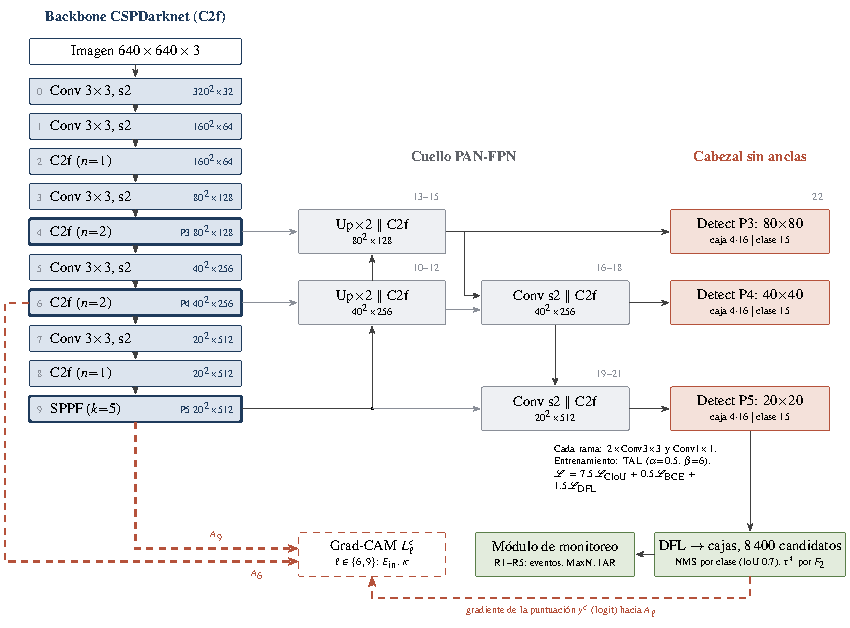
\includegraphics[width=.86\linewidth]{figuras/arquitectura.pdf}
  \caption{YOLOv8-s ajustado a las 15 clases de CCT-20. Los índices grises numeran las capas; \(\Vert\) denota concatenación por canales. Las flechas discontinuas marcan las activaciones \(A_6\) y \(A_9\) y el gradiente de la puntuación de clase usados por Grad-CAM (\cref{sec:gradcam}).}
  \label{fig:arquitectura}
\end{figure}

La asignación de candidatos a verdades de terreno sigue a \textcite{feng2021tood}: para cada par se calcula
\begin{equation}
  t = s^{\alpha}\, u^{\beta}, \qquad \alpha = 0.5,\ \beta = 6,
  \label{eq:tal}
\end{equation}
con \(s\) la puntuación de la clase verdadera y \(u\) el IoU de la caja predicha, y a cada objeto se asignan los \(k_{\mathrm{TAL}} = 10\) candidatos de mayor \(t\). La función objetivo es
\begin{equation}
  \mathcal{L} = \lambda_{\mathrm{box}}\,\mathcal{L}_{\mathrm{CIoU}} + \lambda_{\mathrm{cls}}\,\mathcal{L}_{\mathrm{BCE}} + \lambda_{\mathrm{dfl}}\,\mathcal{L}_{\mathrm{DFL}},
  \qquad (\lambda_{\mathrm{box}}, \lambda_{\mathrm{cls}}, \lambda_{\mathrm{dfl}}) = (7.5,\ 0.5,\ 1.5),
  \label{eq:perdida}
\end{equation}
con la pérdida de regresión de \textcite{zheng2020ciou},
\begin{equation}
  \mathcal{L}_{\mathrm{CIoU}} = 1 - \IoU + \frac{\rho^2(\mathbf{b}, \mathbf{b}^{\mathrm{gt}})}{c^2} + \alpha_v v, \quad
  v = \frac{4}{\pi^2}\Big(\arctan\frac{w^{\mathrm{gt}}}{h^{\mathrm{gt}}} - \arctan\frac{w}{h}\Big)^2, \quad
  \alpha_v = \frac{v}{(1-\IoU) + v},
  \label{eq:ciou}
\end{equation}
donde \(\rho\) es la distancia entre centros y \(c\) la diagonal de la caja envolvente mínima. La pérdida focal distribucional \parencite{li2020gfl} concentra la masa de cada lado en los enteros \(y_i \le y < y_{i+1}\) que rodean al objetivo \(y\):
\begin{equation}
  \mathcal{L}_{\mathrm{DFL}}(S_i, S_{i+1}) = -\big[(y_{i+1}-y)\log S_i + (y-y_i)\log S_{i+1}\big].
  \label{eq:dfl}
\end{equation}
Un candidato no asignado solo contribuye a \(\mathcal{L}_{\mathrm{BCE}}\), con objetivo cero en las 15 clases; esa es la supervisión del fondo, sin una clase \emph{empty}.

\subsection{Decisiones de entrenamiento y tratamiento del fondo}
\label{sec:decisiones}
La \cref{tab:hiper} (apéndice) resume las decisiones. Tres responden a propiedades del dominio. \Textcite{beery2018} usaron la inversión horizontal como único aumento; aquí se conserva y se excluyen la inversión vertical y la rotación, porque la gravedad fija la orientación de los animales y la cámara no se mueve. Las capturas nocturnas son infrarrojas y monocromas, de modo que la perturbación de tono carece de significado físico y se anula. El mosaico \parencite{bochkovskiy2020} diversifica el contexto de cada animal, una presión directa contra el atajo de fondo, y se desactiva en las 10 últimas épocas.

El diseño preveía incorporar imágenes vacías como negativos explícitos hasta una fracción \(f = \fracFondo\,\%\), muestreadas por cámara. La auditoría mostró que el \texttt{train} oficial de CCT-20 contiene 12\,099 imágenes con caja, 1\,454 con animal sin caja y ninguna vacía. A se mantuvo fiel al protocolo oficial, sin importar vacías de otras cámaras. Para que la ablación aislara el efecto de las cámaras y no el del fondo, B usó la misma fracción, \(f_A = 0\). En ambos modelos la supervisión del fondo procede, por tanto, de las regiones sin animal de las imágenes con fauna. Su magnitud se acota con la siguiente proposición.

\begin{proposicion}
\label{prop:fondo}
Sea una imagen con \(n\) objetos y \(N = 8\,400\) candidatos. Con la asignación de \textcite{feng2021tood}, que asigna como máximo \(k_{\mathrm{TAL}}\) candidatos por objeto, la fracción de candidatos supervisados como fondo es al menos \(1 - k_{\mathrm{TAL}}\,n/N\).
\end{proposicion}
\begin{proof}
Cada objeto selecciona a lo sumo \(k_{\mathrm{TAL}}\) candidatos, y un candidato asignado a varios objetos se conserva para uno solo, luego hay a lo sumo \(k_{\mathrm{TAL}}\,n\) positivos. Los \(N - k_{\mathrm{TAL}}\,n\) restantes reciben objetivo nulo en \(\mathcal{L}_{\mathrm{BCE}}\) (\cref{eq:perdida}).
\end{proof}
Con \(\bar n = \nCajasTrainA/\nTrainA \approx 1.04\) cajas por imagen en A, la cota da más de un 99.8\,\% de candidatos de fondo por imagen. Lo que falta no es supervisión negativa sino diversidad de escenas vacías, como viento, vegetación o cambios de luz. Sus consecuencias se miden con la tasa de falsos positivos en vacías (\cref{sec:res-cistrans}), y las vacías intervienen explícitamente en la validación (24.8\,\% de las \nVal\ imágenes), en la selección del umbral y en todas las métricas de prueba. B suma \nUbicTrainB\ cámaras y \nCajasTrainB\ cajas, frente a \nUbicTrainA\ cámaras y \nCajasTrainA\ cajas de A: solo 46 de las \nUbicExtTrain\ cámaras externas contienen cajas de las 15 clases (\cref{tab:entrenamiento}, apéndice). Ambos se seleccionan con \(\texttt{cis\_val}\cup\texttt{trans\_val}\) y parada temprana de paciencia 15.



\subsection{Protocolo de evaluación}
\label{sec:evaluacion}
Una detección \(\hat{b}\) empareja con una caja verdadera \(b\) de la misma clase si \(\IoU(\hat{b}, b) = |\hat{b} \cap b|/|\hat{b} \cup b| \ge t\). Siguiendo a \textcite{lin2014coco}, las detecciones se procesan en orden decreciente de puntuación con emparejamiento único. Con la precisión interpolada \(\tilde{p}(r) = \max_{r' \ge r} p(r')\),
\begin{equation}
  \begin{gathered}
  \mathrm{AP}_{c,t} = \frac{1}{101} \sum_{r \in \{0, 0.01, \dots, 1\}} \tilde{p}(r), \\
  \mAP@0.5 = \frac{1}{|C|}\sum_{c} \mathrm{AP}_{c,0.5}, \qquad
  \mAP@0.5{:}0.95 = \frac{1}{10|C|}\sum_{c}\sum_{t\in T} \mathrm{AP}_{c,t},
  \end{gathered}
  \label{eq:map}
\end{equation}
con \(T = \{0.50, 0.55, \dots, 0.95\}\). \Textcite{beery2018} consideran IoU \(\ge 0.5\) el criterio adecuado para CCT dada la variabilidad entre anotadores \parencite{everingham2010}; se reportan ambas métricas. Las predicciones usan puntuación mínima \(10^{-3}\), NMS por clase con IoU 0.7 y 100 detecciones por imagen.

\paragraph{Ponderación de las vacías del trans ampliado.} De las cerca de 18\,000 vacías de las 30 cámaras externas de validación se descarga una de cada \(k = \kVacias\) por cámara, y cada una se pondera por \(k\). Para cualquier estadístico aditivo sobre imágenes \(S = \sum_i g(i)\), como los conteos de verdaderos y falsos positivos que forman la curva precisión-recall, el estimador de Horvitz-Thompson
\begin{equation}
  \hat{S} = \sum_{i \in \mathcal{M}} \frac{g(i)}{\pi_i}, \qquad \pi_i = \begin{cases} 1/k & \text{si } i \text{ es vacía},\\ 1 & \text{en otro caso},\end{cases}
  \label{eq:ht}
\end{equation}
es insesgado, \(\mathbb{E}[\hat S] = S\), porque cada imagen entra en la muestra \(\mathcal{M}\) con probabilidad \(\pi_i\). Tras la ponderación, las vacías representan el \pctVaciasExtPond\,\% de las \nTransExt\ imágenes evaluadas. La cifra supera al \pctVaciasExtVal\,\% del total porque las imágenes con animal sin caja, el 38\,\% de esas cámaras, no admiten evaluación por cajas.

\paragraph{Brecha e intervalos.} La brecha se expresa en puntos y como incremento relativo del error \parencite{beery2018},
\begin{equation}
  \Delta = \mAP_{\mathrm{cis}} - \mAP_{\mathrm{nuevo}}, \qquad
  \Delta_{\mathrm{rel}} = \frac{1-\mAP_{\mathrm{nuevo}}}{1-\mAP_{\mathrm{cis}}} - 1 .
  \label{eq:brecha}
\end{equation}
Los intervalos al 95\,\% se obtienen con \emph{bootstrap} de percentiles \parencite{efron1993}, remuestreando cámaras con reemplazo (\(B = 300\)), porque las imágenes de una cámara no son independientes. En cada réplica se aplica la misma muestra de cámaras a A y a B, lo que produce un intervalo pareado para la mejora \(\mAP_B - \mAP_A\). El evaluador se implementó desde cero para admitir pesos y subgrupos ignorados, y su salida coincide con \texttt{pycocotools} hasta la última cifra (\cref{tab:verificacion}, apéndice).

\paragraph{Umbral de operación.} Cada modelo opera con
\begin{equation}
  \tau^\ast = \argmax_{\tau}\, F_{2}(\tau), \qquad F_\beta = \frac{(1+\beta^2)\,P R}{\beta^2 P + R},
  \label{eq:fbeta}
\end{equation}
elegido en validación, con \(\beta = 2\) para ponderar el recall cuatro veces más que la precisión \parencite{vanrijsbergen1979}. Resulta \(\tau^\ast_A = \tauFdosA\) y \(\tau^\ast_B = \tauFdosB\), frente a \(\tauFunoA\) y \(\tauFunoB\) si se maximizara \(F_1\). La asimetría se fundamenta en la \cref{sec:discusion}.

\subsection{Dependencia del fondo: Grad-CAM y contrafactual}
\label{sec:gradcam}
Para una caja verdadera \(b\) de clase \(c\), se elige entre los 8\,400 candidatos el de mayor puntuación de \(c\) con IoU \(\ge 0.3\) respecto de \(b\), y su \emph{logit} \(y^c\) se retropropaga hasta la activación \(A_\ell \in \mathbb{R}^{K\times H\times W}\) \parencite{selvaraju2017}:
\begin{equation}
  \alpha^c_k = \frac{1}{HW}\sum_{i,j} \frac{\partial y^c}{\partial A^{k}_{\ell,ij}}, \qquad
  L^c_\ell = \mathrm{ReLU}\Big(\sum_{k} \alpha^c_k A^{k}_{\ell}\Big),
  \label{eq:gradcam}
\end{equation}
con \(\ell = 9\) (SPPF, paso 32, la última capa de la red troncal) y \(\ell = 6\) (C2f, paso 16) como verificación de resolución. Se definen
\begin{equation}
  E_{\mathrm{in}} = \frac{\sum_{p\in b} L^c_\ell(p)}{\sum_{p\in I} L^c_\ell(p)}, \qquad
  \kappa = \frac{E_{\mathrm{in}}}{|b|/|I|}.
  \label{eq:kappa}
\end{equation}

\begin{proposicion}
\label{prop:kappa}
Sea \(\mu_S\) la media de \(L^c_\ell\) sobre la región \(S\). Entonces \(\kappa = \mu_b/\mu_I\); además \(\kappa > 1\) si y solo si \(\mu_b > \mu_{I\setminus b}\), y \(\kappa \le |I|/|b|\).
\end{proposicion}
\begin{proof}
De la \cref{eq:kappa}, \(E_{\mathrm{in}} = |b|\mu_b / (|I|\mu_I)\), luego \(\kappa = \mu_b/\mu_I\). Como \(\mu_I = \frac{|b|}{|I|}\mu_b + \frac{|I\setminus b|}{|I|}\mu_{I\setminus b}\) es una combinación convexa con pesos positivos, \(\mu_b > \mu_I \iff \mu_b > \mu_{I\setminus b}\). La cota se sigue de \(E_{\mathrm{in}} \le 1\).
\end{proof}
Por la \cref{prop:kappa}, \(\kappa\le1\) indica que la evidencia de la clase no está más concentrada en el animal que en el resto de la escena. La cota implica que las cajas grandes empujan \(\kappa\) hacia 1 por construcción, de modo que solo se comparan dominios con distribuciones de tamaño parecidas. Las mismas 250 cajas por dominio se analizan con A y con B, y los regímenes se comparan con la prueba de Mann--Whitney \parencite{mann1947}.

\paragraph{Contrafactual de fondo.} La mediana píxel a píxel de las vacías de la cámara \(\ell\) en el modo de captura \(m\in\{\text{color},\text{IR}\}\),
\begin{equation}
  B_{\ell,m}(p) = \med_{j \in \mathcal{V}_{\ell,m}} I_j(p), \qquad |\mathcal{V}_{\ell,m}| \le 40,
  \label{eq:fondo-mediana}
\end{equation}
estima su fondo. En imágenes con un único animal, la caja ampliada un 10\,\% se sustituye por \(\gamma \odot B_{\ell,m}\), con \(\gamma\) la razón de medianas por canal fuera de la caja. La \emph{persistencia} es la fracción de casos detectados a \(\tau^\ast\) que mantienen una detección de la misma especie (IoU \(\ge 0.3\), puntuación \(\ge\tau^\ast\)) sin el animal. Como tercera prueba se reporta la tasa de falsos positivos en vacías, FPR\(_\varnothing\), y el AUROC de la puntuación máxima por imagen entre vacía y fauna; este último no depende del umbral y permite comparar A con B.

\subsection{Oclusión y tamaño}
\label{sec:oclusion}
CCT no anota oclusión. La visibilidad \(v\) es la fracción de píxeles de la caja que difieren del fondo de la cámara:
\begin{equation}
  \begin{gathered}
  v = \frac{1}{|b|}\sum_{p\in b} \mathbb{1}\big[D(p) > \theta\big], \qquad
  D = G_{\sigma} * \big| I - \gamma B_{\ell,m} \big|, \\
  \theta = \max\big(12,\ \med(D_{\bar b}) + 3 \cdot 1.4826\,\mathrm{MAD}(D_{\bar b})\big),
  \end{gathered}
  \label{eq:visibilidad}
\end{equation}
con \(\bar b\) el complemento de las cajas. Una caja ocupada por vegetación o roca reproduce el fondo y tiene \(v\) bajo. Normalizando con el percentil 75 por especie, \(v_{75}(c)\),
\begin{equation}
  o = \max\Big(\underbrace{\clip\big(1 - v/v_{75}(c),\,0,\,1\big)}_{o_{\mathrm{vis}}},\ \underbrace{0.5\,\mathbb{1}[\eta = 1] + 0.8\,\mathbb{1}[\eta \ge 2]}_{o_{\mathrm{tr}}},\ \underbrace{\max_{b'\neq b} |b\cap b'|/|b|}_{o_{\mathrm{sol}}}\Big),
  \label{eq:oclusion}
\end{equation}
donde \(\eta\) es el número de bordes del encuadre que toca la caja. Los niveles son bajo \([0, 1/3)\), medio \([1/3, 2/3)\) y alto \([2/3, 1]\). Como \(o_{\mathrm{vis}}\) puede confundir oclusión y camuflaje \parencite{beery2018}, el estimador se contrasta con \nValOcl\ cajas etiquetadas a ciegas por un modelo multimodal \parencite{anthropic2026claude} y revisadas a mano (\cref{sec:val-oclusion}), con el \(\kappa_w\) cuadrático de \textcite{cohen1968}.
El tamaño se mide a la resolución de entrada con los umbrales de COCO \parencite{lin2014coco}: pequeño si el área es menor que \(32^2\) px, mediano si es menor que \(96^2\) y grande en el resto. En cada subgrupo se ignoran las cajas ajenas. El indicador principal es el recall a \(\tau^\ast\), R@\(\tau^\ast\), que no depende de cómo se atribuyan los falsos positivos a los subgrupos.

\subsection{Módulo de monitoreo ecológico}
\label{sec:monitoreo}
El módulo transforma detecciones por fotograma en un reporte de actividad mediante cinco reglas. \textbf{R1}: se conservan las detecciones con puntuación \(\ge \tau^\ast\). \textbf{R2}: NMS agnóstico a la especie con IoU 0.6, para no contar un individuo como dos especies. \textbf{R3}: un fotograma sin detecciones es vacío; en otro caso registra el número de individuos \(n_k\) por especie. \textbf{R4}: dos registros de una especie pertenecen a eventos distintos si
\begin{equation}
  t_k - t_{k-1} > \Delta_{\mathrm{ind}} = 30\ \text{min},
  \label{eq:evento}
\end{equation}
el criterio de independencia de \textcite{obrien2003} recomendado por \textcite{meek2014}. \textbf{R5}: cada evento \(e\) se resume con \(\mathrm{MaxN}_e = \max_{k\in e} n_k\), y cada especie con el índice de abundancia relativa \(\mathrm{IAR} = 100\, N_{\mathrm{ev}}/D\), con \(D\) los días de operación. El reporte se agrega por madrugada [0, 6) h, mañana [6, 12) h, tarde [12, 18) h y noche [18, 24) h. Se demuestra sobre el flujo completo de la cámara del trans ampliado de mayor riqueza etiquetada: la cámara \locDemo, con \fotogramasDemo\ fotogramas en \diasDemo\ días, que ningún modelo vio. El mismo módulo aplicado a las etiquetas verdaderas produce la referencia.

\subsection{Extensión entre conjuntos de datos}
\label{sec:ena24}
Se evaluaron A y B sin reentrenar sobre ENA24-detection \parencite{yousif2019}: \nEna\ imágenes del este de Norteamérica con \nCajasEna\ cajas, de un bosque templado caducifolio y con otro hardware de captura. A diferencia de conjuntos neotropicales como Orinoquía \parencite{velez2023}, tiene cajas en todas sus imágenes, lo que permite el mismo mAP, y comparte \nClasesEna\ de las 15 clases. Cada taxón \(s\) se asigna a la clase más específica que lo contiene,
\begin{equation}
  m(s) = \argmax_{c \in C:\ s \preceq c}\ \mathrm{prof}(c),
  \label{eq:mapeo}
\end{equation}
con \(s \preceq c\) la pertenencia al clado de \(c\). Así, \emph{Tamias} y \emph{Marmota} (Sciuridae) van a \texttt{squirrel}. En la ejecución reportada, la implementación por subcadenas asignó \emph{Sciurus niger} (\emph{eastern fox squirrel}) a \texttt{fox}; el cuaderno corrige el orden de las reglas, y el efecto se limita a las clases \texttt{fox} y \texttt{squirrel} de ENA24. Los taxones sin clase contenedora (\pctNoMapeadas\,\% de las cajas) no son verdad de terreno de ninguna clase, pero las detecciones sobre ellos cuentan como falsos positivos. Además se reporta un AP agnóstico a la especie, AP\(^{\mathrm{agn}}_{50}\), que aísla la localización.

% =====================================================================
\section{Resultados}
\label{sec:resultados}

\subsection{Desempeño global y por especie}
\label{sec:res-especie}
La parada temprana detuvo A en la época \epocasRealA\ y B en la \epocasRealB, y B alcanzó pérdidas de validación menores en los tres términos (\cref{fig:curvas}, apéndice). La \cref{tab:global} resume los cuatro dominios. En cis, A alcanza un mAP@0.5 de \mapCisCincA\,\% (IC 95\,\% [\icCisALo, \icCisAHi]) y B de \mapCisCincB\,\% ([\icCisBLo, \icCisBHi]), una mejora pareada de \mejoraCis\ puntos ([\icMejoraCisLo, \icMejoraCisHi]). Ambas cifras quedan por debajo del 77\,\% de Faster R-CNN \parencite{beery2018}, entrenado a mayor resolución (lado mayor de 1024 px) y con dos etapas.

\begin{table}[h!]
  \centering
  \caption{Desempeño por dominio y modelo. AP\(^{\mathrm{agn}}_{50}\): AP agnóstico a la especie. Las columnas centrales descomponen las cajas verdaderas al umbral \(\tau^\ast\) de cada modelo. FPR\(_\varnothing\): fracción de vacías con alguna detección \(\ge\tau^\ast\) (ENA24 no tiene vacías).}
  \label{tab:global}
  \small\tabres{tab_global}
\end{table}

La \cref{tab:especies} desagrega el AP@0.5 por especie. En A, el desbalance determina el desempeño: la correlación de Spearman \parencite{spearman1904} entre \(\mathrm{AP}_{c,0.5}\) y \(\log_{10} n_{\mathrm{train},c}\) es \(\rho = \rhoCisA\) (\(p = \pCisA\)) en cis y \(\rhoTransA\) (\(p = \pTransA\)) en trans. Las especies con menos de 50 cajas (ciervo, tejón, zorro) obtienen entre 0 y 33\,\% en cis, y en trans el AP medio es \apCabezaTransA\,\% en las especies por encima de la mediana de cajas frente a \apColaTransA\,\% en las de debajo. B multiplica por 74 las cajas de ciervo y por 134 las de zorro, y la correlación deja de ser significativa: \(\rho = \rhoCisB\) (\(p = \pCisB\)), \(\rhoTransB\) (\(p = \pTransB\)) y \(\rhoExtB\) en el trans ampliado. La diferencia entre especies frecuentes y raras en trans se reduce de 28.4 a 19.1 puntos (\apCabezaTransB\,\% frente a \apColaTransB\,\%). Los mayores avances se concentran en las especies que más datos ganaron, como ciervo (cis: de 32.8 a 65.5\,\%), roedor y zorro en el trans ampliado (\cref{fig:ap-instancias}). En cambio, aves y roedores siguen por debajo del 10\,\% en trans, y la ardilla no se detecta en el trans ampliado con ninguno de los modelos. Son especies pequeñas y miméticas, cuya escasa señal visual no compensa el volumen de datos.

\begin{table}[h!]
  \centering
  \caption{AP@0.5 por especie (\%) para A y B en cada dominio, con el número de cajas de entrenamiento \(n_{\mathrm{train}}\) de cada modelo. ``--'': especie ausente del dominio.}
  \label{tab:especies}
  \small\tabres{tab_especies}
\end{table}

\begin{figure}[h!]
  \centering
  \figres[.6\linewidth]{fig_ap_vs_instancias}
  \caption{Izquierda: AP@0.5 por especie del modelo A frente a sus cajas de entrenamiento. Derecha: desplazamiento de cada especie de A (origen) a B (punta) en los dos dominios de cámaras nuevas.}
  \label{fig:ap-instancias}
\end{figure}

\subsection{Generalización entre cámaras}
\label{sec:res-cistrans}
\begin{table}[h!]
  \centering
  \caption{Brecha entre cámaras vistas y nuevas (\cref{eq:brecha}), con IC por \emph{bootstrap} de cámaras.}
  \label{tab:brecha}
  \small\tabres{tab_brecha}
  \vspace{2mm}
  \caption{Pruebas de dependencia del fondo. \(\tilde\kappa_\ell\): concentración mediana de Grad-CAM en la capa \(\ell\) (\cref{eq:kappa}); \(\tilde E_{\mathrm{in}}\): fracción mediana de energía en la caja (capa 9); persistencia: detecciones que sobreviven al reemplazo del animal por el fondo de su cámara.}
  \label{tab:fondo}
  \small\tabres{tab_fondo}
\end{table}

La \cref{tab:brecha} reporta la brecha de cada modelo. En A, frente a las 9 cámaras trans, \(\Delta = \brechaTransA\) puntos (IC 95\,\% [\icBrechaTransALo, \icBrechaTransAHi]) y \(\Delta_{\mathrm{rel}} = \incrErrorTransA\)\,\%, casi el triple del 28\,\% de Faster R-CNN \parencite{beery2018}. Frente al trans ampliado, la brecha llega a \brechaExtA\ puntos ([\icBrechaExtALo, \icBrechaExtAHi]). Al añadir cámaras, B mejora en trans \mejoraTrans\ puntos ([\icMejoraTransLo, \icMejoraTransHi]), pero como también mejora en cis su brecha queda en \brechaTransB\ puntos ([\icBrechaTransBLo, \icBrechaTransBHi]). En el trans ampliado, en cambio, la mejora es de \mejoraExt\ puntos ([\icMejoraExtLo, \icMejoraExtHi]) y la brecha se reduce a \brechaExtB\ puntos, porque esas cámaras se parecen más a las externas incorporadas en B que a las de CCT-20. B también uniformiza el desempeño entre cámaras: el coeficiente de variación del mAP por cámara baja de \cvTransA\ a \cvTransB\ en trans y de \cvExtA\ a \cvExtB\ en el trans ampliado (\cref{fig:ubicacion}, apéndice). Estos resultados confirman la hipótesis de \textcite{schneider2020}.

La comparación con el AP agnóstico localiza el fallo. En trans, A localiza el \agnTransA\,\% de los animales pero solo alcanza un \mapTransCincA\,\% de mAP por clase. A \(\tau^\ast\), el \confuTransA\,\% de las cajas se localiza con la especie equivocada y el \omitTransA\,\% se omite. Como observaron \textcite{beery2018}, la clasificación es más frágil que la detección frente al cambio de cámara. En el trans ampliado, A pierde además la localización (AP\(^{\mathrm{agn}}_{50} = \agnExtA\,\%\), \omitExtA\,\% de omisiones), y B la recupera hasta \agnExtB\,\%.


\paragraph{Evidencia sobre el aprendizaje del fondo.} La \cref{tab:fondo} reúne las tres pruebas. La más concluyente es la separabilidad entre vacías y fauna, independiente del umbral. En A, el AUROC cae de \aucCisA\ en cis a \aucTransA\ en trans y \aucExtA\ en el trans ampliado. Al mismo umbral, la tasa de falsos positivos en vacías pasa de \fprVaciasCisA\,\% a \fprVaciasTransA\,\%: el detector responde al fondo de cámaras que no conoce con la misma confianza que a un animal. B mantiene el AUROC en \aucCisB, \aucTransB\ y \aucExtB, de modo que la diversidad de cámaras estabiliza el rechazo del fondo.

\begin{figure}[h!]
  \centering
  \figres[.72\linewidth]{fig_gradcam_ejemplos}
  \caption{Mapas Grad-CAM de la capa 9 del modelo B en cámaras vistas y nuevas, con la caja verdadera en verde.}
  \label{fig:gradcam}
\end{figure}

Grad-CAM apunta en la misma dirección. La concentración mediana en la capa 9 es menor que 1 en todos los casos (\cref{fig:kappa}, apéndice), y los mapas de la \cref{fig:gradcam} resaltan con frecuencia vegetación, bordes del encuadre y zonas iluminadas antes que al animal. En A, \(\tilde\kappa\) baja de \kCisProfA\ en cis a \kTransProfA\ en trans (Mann--Whitney \(p = \pKTransProfA\)). En B, la concentración es mayor en ambos dominios (\kCisProfB\ y \kTransProfB). El trans ampliado se excluye de esta comparación porque sus cajas grandes acercan \(\kappa\) a 1 (\cref{prop:kappa}). El contrafactual muestra que la detección desaparece casi siempre al retirar al animal en cis y trans (persistencia de \persistCisA\ y \persistTransA\,\% en A, nula en B). El detector usa al animal cuando lo detecta, y la dependencia del contexto se manifiesta sobre todo como falsos positivos en escenas vacías desconocidas. La persistencia de B en el trans ampliado (\persistExtB\,\%) no se interpreta, porque allí predominan cajas que ocupan casi todo el encuadre y dejan sin contexto el cálculo de \(\gamma\).


\subsection{Robustez ante oclusión y tamaño}
\label{sec:res-oclusion}
\begin{table}[h!]
  \centering
  \caption{Recall a \(\tau^\ast\) (\%) por nivel estimado de oclusión y por tamaño (umbrales de COCO a \imgsz\ px).}
  \label{tab:oclusion}
  \small\tabres{tab_oclusion_tamano}
\end{table}

El tamaño domina sobre la oclusión (\cref{tab:oclusion}; \cref{fig:oclusion}, apéndice). Las cajas pequeñas son raras (1 a 3\,\% del total), pero su recall a \(\tau^\ast\) es de \recPeqCisA\,\% en cis y \recPeqTransA\,\% en trans con A, frente a más del 80\,\% de las grandes en cis. La caída entre grandes y pequeñas es de \caidaTamCisA\ y \caidaTamTransA\ puntos. B mejora las pequeñas en trans hasta \recPeqTransB\,\% sin cerrar la diferencia. Esto es coherente con la resolución de 640 px, que reduce un animal lejano de una imagen de 1024 px a pocas celdas de paso 8. La oclusión estimada tiene un efecto monótono pero moderado: entre los niveles bajo y alto, el recall de A cae \caidaOclCisA\ puntos en cis y \caidaOclTransA\ en trans, y el de B, \caidaOclCisB\ y \caidaOclTransB. Sin embargo, el estimador infla el nivel alto, sobre todo en tomas nocturnas de bajo contraste (\(\kappa_w = \kappaOcl\), IC 95\,\% [\kappaOclLo, \kappaOclHi]; \cref{sec:val-oclusion}), de modo que esa caída mezcla oclusión y baja visibilidad.


\subsection{Módulo de monitoreo}
\label{sec:res-monitoreo}
En la cámara \locDemo, la referencia registra \eventosReal\ eventos independientes de \especiesReal\ especies. El módulo produce \eventosA\ eventos de \especiesA\ especies con A y \eventosB\ de \especiesB\ con B (\cref{tab:mon-resumen,tab:mon-especies}). El total de A coincide por compensación de errores. Ningún modelo registra los 16 eventos de lagartija, una especie ausente del espacio de etiquetas, y ambos subestiman la ardilla (5 eventos frente a 13). A cambio, A inventa 10 eventos de coyote y 6 de conejo, y B 19 de ciervo y 5 de coyote. Por eso el error agregado por especie es del \errEventosA\,\% con A y del \errEventosB\,\% con B. La fracción de fotogramas sin fauna sube de \vaciosReal\,\% en la referencia a \vaciosA\,\% y \vaciosB\,\% según los módulos. El lince conserva su patrón nocturno, aunque B lo sobreestima (\cref{fig:actividad}, apéndice). La especie ajena al espacio de etiquetas desaparece del reporte sin señal de alerta.

\begin{table}[h!]
  \centering
  \begin{minipage}[t]{.42\linewidth}\centering
    \caption{Resumen de la cámara \locDemo.}
    \label{tab:mon-resumen}
    \footnotesize\tabres{tab_monitoreo_resumen}
  \end{minipage}\hfill
  \begin{minipage}[t]{.55\linewidth}\centering
    \caption{Eventos por especie y periodo: modelo B (referencia); última columna: eventos de A.}
    \label{tab:mon-especies}
    \footnotesize\tabres{tab_monitoreo_especies}
  \end{minipage}
\end{table}

\subsection{Generalización a otra región}
\label{sec:res-ena24}
Sobre ENA24, A alcanza un mAP@0.5 de \mapEnaCincA\,\% y B de \mapEnaCincB\,\% (IC 95\,\% por \emph{bootstrap} de imágenes: [\icEnaALo, \icEnaAHi] y [\icEnaBLo, \icEnaBHi]). El AP agnóstico es mucho mayor, \agnEnaA\,\% y \agnEnaB\,\%: ambos detectores encuentran a los animales del otro bioma pero fallan al nombrarlos. A \(\tau^\ast\), A confunde la especie en el \confuEnaA\,\% de las cajas y B en el \confuEnaB\,\% (\cref{fig:confusion}, apéndice). A, con 44 cajas de entrenamiento, clasifica como coyote el 49\,\% de los ciervos de cola blanca (AP de 0.1\,\%). B, que vio ciervos de las cámaras externas, alcanza un AP de 52.4\,\% aunque la especie oriental es otra.

% =====================================================================
\section{Discusión}
\label{sec:discusion}
\paragraph{Uso responsable de la IA en conservación.} Los dos tipos de error no tienen el mismo costo. Un falso positivo consume minutos de revisión de un especialista. Un falso negativo de una especie amenazada la retira del registro: su ocupación y su abundancia relativa se subestiman, y las decisiones de manejo se toman sin ella. Como la revisión humana corrige los falsos positivos pero nadie revisa lo que el sistema descartó, la asimetría justifica operar a alto recall. De ahí la elección de \(\tau^\ast\) por \(F_2\) (\cref{eq:fbeta}), que en validación da un recall de \recTauB\,\% con una precisión de \precTauB\,\% en B, y la recomendación de enviar a revisión toda detección entre \(\tau^\ast\) y \(\tau_{F_1}\), además de toda secuencia con una especie de interés.

El segundo riesgo es desplegar el detector en otra región sin validación local: ni 46 cámaras adicionales cerraron la brecha frente a las trans. En la Amazonía y los Andes peruanos, la fauna objetivo (tapir, pecarí, jaguar, oso de anteojos) no pertenece al espacio de etiquetas, y el caso de la lagartija muestra que el detector la omitirá o la asignará a la clase visualmente más cercana sin señal de incertidumbre. El sotobosque denso agrava además la oclusión y reduce el tamaño aparente. Un despliegue responsable exige validación etiquetada en las cámaras de destino, recalibrar \(\tau^\ast\) y abstenerse ante especies fuera del espacio de etiquetas. La brecha entre AP\(^{\mathrm{agn}}_{50}\) y mAP en ENA24 (cerca de 50 puntos en B) respalda la alternativa de dos etapas: un detector agnóstico seguido de un clasificador regional \parencite{beery2019megadetector,shepley2021}.

\paragraph{Limitaciones.} (1) El \texttt{train} oficial no contiene vacías y B replicó esa fracción, de modo que ningún modelo vio escenas vacías. (2) B difiere de A en número de cámaras y en composición de especies; la mitad de las cajas del trans ampliado es de ciervo, y la ablación no separa ambos efectos. (3) El estimador de oclusión sobrestima el nivel en tomas de bajo contraste (\cref{sec:val-oclusion}). (4) Grad-CAM tiene resolución gruesa en la capa 9, y tanto \(\kappa\) como el contrafactual dependen del tamaño de la caja. (5) Se usó una semilla, 640 px y evaluación por fotograma. (6) ENA24 carece de ubicaciones y de vacías, y el mapeo asignó \emph{Sciurus niger} a \texttt{fox}.

% =====================================================================
\section{Conclusiones}
\label{sec:conclusiones}
Con el protocolo oficial, YOLOv8-s alcanza \mapCisCincA\,\% de mAP@0.5 en cámaras vistas y \mapTransCincA\,\% en nuevas; la caída se concentra en la clasificación y en el rechazo del fondo. Añadir cámaras externas mejora todos los dominios y atenúa el efecto del desbalance, sin cerrar la brecha frente a las cámaras trans. El tamaño del objeto domina la dificultad, y un monitoreo con totales correctos puede ocultar errores de composición.

\printbibliography[title=Referencias]

% =====================================================================
\appendix
\section{Material complementario}
\label{sec:apendice}
\subsection{Validación del estimador de oclusión}
\label{sec:val-oclusion}
La muestra de validación contiene \nValOcl\ cajas de \texttt{cis\_test}, \texttt{trans\_test} y el trans ampliado, 40 por nivel estimado. La anotación siguió dos etapas. Primero, el anotador multimodal etiquetó cada recorte sin acceso al nivel estimado, según la fracción visible del cuerpo: bajo si se observa más de dos tercios del animal, medio entre uno y dos tercios, y alto por debajo de un tercio. La vegetación, las rocas, otros individuos y el borde del encuadre cuentan como oclusión; el camuflaje y la oscuridad, no. Después, los autores revisaron manualmente las \nValOcl\ etiquetas con el mismo criterio y las ratificaron sin cambios. Frente a esa referencia, el acuerdo es leve en la escala de \textcite{landis1977}: \(\kappa_w = \kappaOcl\), con IC 95\,\% [\kappaOclLo, \kappaOclHi] por \emph{bootstrap} de cajas, coincidencia exacta del \accOcl\,\% y discrepancia de a lo sumo un nivel en el \accAdyOcl\,\%. La correlación de rangos es positiva pero débil (\(\rho = \rhoOcl\), \(p = \pRhoOcl\)).

El error es asimétrico (\cref{tab:val-oclusion}). El estimador asigna un nivel superior al anotado en el \sobreOcl\,\% de las cajas y uno inferior en el \subOcl\,\%, y la mitad de las cajas que clasifica como de oclusión alta muestran al animal casi completo. Esas cajas tienen un contraste interno, medido como la desviación típica de la intensidad del recorte, con mediana \sdAltoBajo, frente a \sdAltoResto\ en el resto del nivel alto (Mann--Whitney \(p = \pSdOcl\)). En el tercil de menor contraste la sobrestimación alcanza el \sobreTerInf\,\% de las cajas, frente al \sobreTerMed\,\% del tercil central. El término \(o_{\mathrm{vis}}\) de la \cref{eq:oclusion} interpreta como oclusión la escasa diferencia con el fondo propia de las tomas infrarrojas nocturnas, en las que el animal es visible pero apenas se separa del fondo. Una versión corregida del estimador debería normalizar \(D\) por el contraste local o sustituir \(o_{\mathrm{vis}}\) por una segmentación del animal.

La referencia tiene límites que deben declararse. Los recortes se juzgaron a unos 60 px de lado y sin la imagen completa, solo con la indicación de contacto con el borde del encuadre. La revisión manual partió de las etiquetas propuestas, lo que puede introducir un sesgo de anclaje hacia ellas. Las 12 primeras cajas no se anotaron a ciegas; excluirlas apenas modifica el resultado (\(\kappa_w = \kappaOclCiega\)). Por último, el \pctSinFondo\,\% de las cajas carece de modelo de fondo, y su nivel depende solo de \(o_{\mathrm{tr}}\) y \(o_{\mathrm{sol}}\).


\begin{figure}[h!]
  \centering
  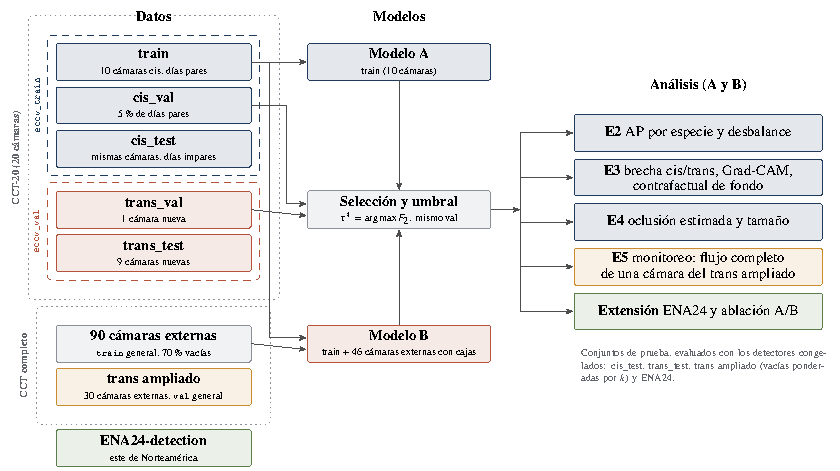
\includegraphics[width=.8\linewidth]{figuras/diseno_experimental.pdf}
  \caption{Diseño experimental. A y B comparten validación, umbral de operación y conjuntos de prueba; solo difieren en las cámaras externas de entrenamiento.}
  \label{fig:diseno}
\end{figure}

\begin{table}[h!]
  \centering
  \caption{Auditoría del conjunto completo de CCT por grupo de cámaras. ``Fuera de clases'': cajas de taxones ajenos a las 15 clases de CCT-20.}
  \label{tab:auditoria}
  \small\tabres{tab_auditoria}
\end{table}

\begin{table}[h!]
  \centering
  \begin{minipage}[t]{.62\linewidth}\centering
  \caption{Hiperparámetros comunes a A y B (Ultralytics 8.3.253).}
  \label{tab:hiper}
  \footnotesize
  \begin{tabular}{@{}p{1.8cm}p{2.5cm}p{3.5cm}@{}}
    \toprule
    Decisión & Valor & Justificación \\
    \midrule
    Inicialización & pesos COCO & Incluye perros, gatos, aves y vehículos \parencite{lin2014coco}. \\
    Resolución & \imgsz\ px & Resolución de preentrenamiento; efecto en objetos pequeños en la \cref{sec:res-oclusion}. \\
    Épocas & 50, paciencia 15 & A: \epocasRealA\ (mejor \mejorEpocaA); B: \epocasRealB\ (mejor \mejorEpocaB). \\
    Optimizador & SGD, \(\eta_0 = 0.01\), momento 0.937, \(\lambda = 5\cdot10^{-4}\), lote 16 & Ajuste fino estándar de YOLOv8. \\
    Color & \(h = 0\), \(s = v = 0.4\) & Sin tono en imágenes infrarrojas. \\
    Geometría & inversión horiz. 0.5; escala 0.5; traslación 0.1 & Cámara fija y orientación gravitatoria. \\
    Mosaico & 1.0; off en las 10 últimas & Contra el atajo de fondo. \\
    MixUp, copy-paste & 0 & Escenas implausibles. \\
    \bottomrule
  \end{tabular}
  \end{minipage}\hfill
  \begin{minipage}[t]{.35\linewidth}\centering
  \caption{Conjuntos de entrenamiento.}
  \label{tab:entrenamiento}
  \footnotesize\tabres{tab_entrenamiento}
  \end{minipage}
\end{table}

\begin{table}[h!]
  \centering
  \caption{Verificación del evaluador propio frente a \texttt{pycocotools} y al \texttt{val()} de Ultralytics. Las diferencias con Ultralytics (entre 1.8 y 3.2 puntos) se deben a su interpolación y emparejamiento, distintos del protocolo COCO.}
  \label{tab:verificacion}
  \small\tabres{tab_verificacion}
\end{table}





\begin{table}[h!]
  \centering
  \caption{Validación del estimador de oclusión: nivel estimado (\cref{eq:oclusion}) frente al nivel anotado en una muestra estratificada de \nValOcl\ cajas. La diagonal, en negrita, corresponde a las coincidencias; las celdas sobre ella, a la subestimación, y las celdas bajo ella, a la sobrestimación.}
  \label{tab:val-oclusion}
  \small\tabres{tab_validacion_oclusion}
\end{table}



\begin{figure}[h!]
  \centering
  \figres[.8\linewidth]{fig_kappa_gradcam}
  \caption{\(\log_{10}\kappa\) por dominio y resultado de la detección; la línea punteada marca la atención uniforme, \(\kappa = 1\).}
  \label{fig:kappa}
\end{figure}

\begin{figure}[h!]
  \centering
  \figres[.49\linewidth]{fig_perdidas}\hfill\figres[.43\linewidth]{fig_map_validacion}
  \caption{Pérdidas de entrenamiento y validación (izquierda) y mAP de validación por época (derecha) de A y B.}
  \label{fig:curvas}
\end{figure}

\begin{figure}[h!]
  \centering
  \figres[.55\linewidth]{fig_map_por_ubicacion}
  \caption{mAP@0.5 por cámara, A frente a B. El tamaño del punto es proporcional al número de imágenes; los puntos sobre la diagonal indican mejora de B.}
  \label{fig:ubicacion}
\end{figure}

\begin{figure}[h!]
  \centering
  \figres{fig_distribucion_clases}
  \caption{Cajas por especie en los conjuntos de entrenamiento de A y B y en los dos conjuntos de cámaras nuevas.}
  \label{fig:distribucion}
\end{figure}



\begin{figure}[h!]
  \centering
  \figres{fig_oclusion_tamano}
  \caption{Recall a \(\tau^\ast\) por nivel de oclusión y por tamaño (línea continua: A; discontinua: B).}
  \label{fig:oclusion}
\end{figure}

\begin{figure}[h!]
  \centering
  \figres{fig_actividad_monitoreo}
  \caption{Eventos independientes por hora en la cámara \locDemo: referencia, módulo con A y módulo con B.}
  \label{fig:actividad}
\end{figure}

\begin{figure}[h!]
  \centering
  \figres{fig_umbral}
  \caption{Precisión, recall, \(F_1\) y \(F_2\) en validación según el umbral, para A y B.}
  \label{fig:umbral}
\end{figure}

\begin{figure}[h!]
  \centering
  \figres{fig_confusion_ext}\\[1mm]
  \figres{fig_confusion_ena24}
  \caption{Matrices de confusión a \(\tau^\ast\), normalizadas por fila, en el trans ampliado (arriba) y en ENA24 (abajo). La última columna recoge las cajas omitidas.}
  \label{fig:confusion}
\end{figure}

\subsection{Reproducibilidad}
Todo el estudio se ejecuta con el cuaderno\\ \texttt{P3\_CamarasTrampa\_YOLOv8.ipynb} (Colab, GPU T4, Ultralytics 8.3.253). Las descargas del conjunto completo, los entrenamientos y las inferencias se reanudan desde Google Drive. Las semillas, las listas de imágenes y el orden de las clases se fijan en la primera ejecución.

\end{document}
